\section{Log jako struktura danych}
    Log jest prostą strukturą danych, a właściwie bazą danych rządząca się kilkoma regułami.
    Możliwe jest dopisywania jedynie do końca pliku, a kolejne wiersze posortowaną są rosnące
    według znacznika czasowego. Innymi słowy wpisy utworzone później znajdą się bliżej końca pliku,
    niż wpisy wcześniejsze. Warto zaznaczyć, że moment, w którym log został wygenerowany nie ma
    nic wspólnego z fizycznym czasem obowiązującym na serwerze. Ważne jest kiedy dane wydarzenia
    miało miejsce, a nie kiedy wpis pojawił się w pliku docelowym.
    
     \begin{figure}[H]
         \centering
         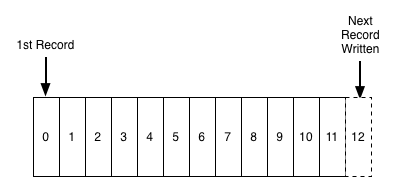
\includegraphics[width=0.80\textwidth]{images/log_file_structure}
         \caption[Log jako struktura danych]{
             Log - struktura danych, źródło: \url{https://content.linkedin.com/content/dam/engineering/en-us/blog/migrated/log.png}
            }
            \label{chapter:logs:history:log_file_as_data_structure_picture}
    \end{figure}

    \subsubsection{Wpisy w logach - kolejne pozycje}
    \label{chapter:logs:history:log_as_data_structure}
    Wpis jako struktura danych przypomina formatem CSV lub FixedLength\footnote{Formaty danych oparte odpowiednio o przecinek, długość kolumny 
        jako separator oddzielający kolejne fragmenty logicznie spójnej informacji \cite{csv_definition}}. 
    Logiczne ułożenie elementów w pojedynczym wierszu jest silnie uzależnione od źródła z którego pochodzi log, 
    a dokładniej z formatu dlań przyjętego. Różnić się będą logi pochodzącego z aplikacji napisanych w języku Python
    lub języka Java. Wynika to jedynie z różnych konwencji przyjętych przez środowisko 
    programistyczne zrzeszone wokół danego języka programowania. Niemniej podstawowe informacje, takie jak:
    \begin{itemize}
        \item znacznik czasowy,
        \item poziom logu,
        \item wiadomość zawarta w logu,
    \end{itemize}
    zawsze się w nim znajdą. 
    
    \begin{figure}[H]
        \centering
        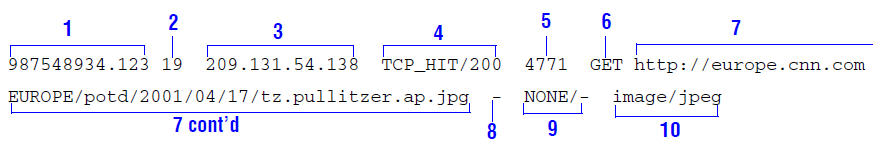
\includegraphics[width=0.80\textwidth]{images/log_data_structure}
        \caption[Wpis w logu jako struktura danych]{
            Wpis - struktura danych, źródło: \url{https://trafficserver.readthedocs.org/en/5.3.x/_images/squid_format.jpg}
        }
        \label{chapter:logs:history:log_as_data_structure_picture}
    \end{figure}
    
    Rysunek \ref{chapter:logs:history:log_as_data_structure_picture} przedstawia przykładowy wpis, który można by znaleźć
    w pliku logów serwera WWW. Poszczególne pola zostały oznaczone numerami i mają następujące znaczenie:
    \begin{enumerate}
        \item Znak czasowy (timestamp) - czas, kiedy klient wykonał żądanie do serwera,
        \item Czas jaki serwer potrzebował na obsłużenie żądania,
        \item Adres IP klienta,
        \item Rezultat z pamięci podręcznej, czy wynik żądania pochodzi z cache'u,
        \item Długość odpowiedzi serwera (ilość danych wysłanych do klienta),
        \item Typ żądania (metoda HTTP) jakie wysłał klient,
        \item URL pod jakiego wystosowano żądania,
        \item Nazwa użytkownika (zalogowanego w kliencie),
        \item Adres proxy, wewnętrzny w strukturze serwera,
        \item Typ odpowiedzi (content-type)
    \end{enumerate}
    
\section{Log, formaty przechowywania}

    \subsection{Pliki tekstowe}
    Pliki tekstowe stanowią najpopularniejszy format przechowywania logów. Najczęściej jest to 
    pierwszy etap, w jakim informacje zawarte w logach mogą być reprezentowane. Jego głównymi zaletami są:
    \begin{itemize}
        \item niski zużycie czasu procesora oraz dysku,
        \item format jest czytelny dla człowieka,
        \item różnorodności formatów przeznaczonych dla wielu języków programowania,
        lub ogólnych, np. \textbf{syslog},
        \item wysoki współczynnik kompresji \cite{logging_log_management}
    \end{itemize}
    
    \subsection{Płaska struktura logów}
    Logi zazwyczaj opisywane są strukturą płaską. Innymi słowy kolejne wpisy nie są ze sobą w żaden sposób
    związane, nie istnieje między nimi żadna relacja. Pliki tekstowe, w których zazwyczaj, aplikacja lub
    urządzania zapisuje logi posiada więc płaską strukturę \cite{logging_log_management}.
    
    \subsection{Binarne pliki logów}
    Jak nazwa wskazuje, logi przechowywane są w formacie binarnym. Główną wadą takiego
    rozwiązania jest brak możliwości odczytania zapisanych danych bez wsparcia odpowiedniego
    oprogramowania oraz wewnętrznego formatu kolejnych wpisów. Innym problem jest mały współczynnik
    skompresowania. Najczęściej udaje się zmniejszyć rozmiar pliku do 10 procent, co w
    porównaniu z plikami tekstowymi stanowi ogromną różnicę.
    Format jest szczególnie znany z dziennika wydarzeń systemów z rodziny Windows \cite{logging_log_management}.
    
    \subsection{Skompresowane pliki logów}
    \label{chapter:logs:history:compressed_log_format}
    Ten format danych nie jest związany z plikami, do których aktualnie zapisywane są dane.
    Jest on jednak szczególnie przydatny dla logów o znaczeniu historycznym. Odpowiednie
    oprogramowanie ma za zadanie utworzenie skompresowanego pliku logu po osiągnięciu przez niego
    odpowiedniego rozmiaru lub upłynięciu określanego czasu. Jedną z takich aplikacji jest 
    \textbf{logrotate}\footnote{Logrotate - \url{http://www.linuxcommand.org/man_pages/logrotate8.html}}.
    Główną zaletą tego formatu jest zwiększenie wolnej przestrzeni dyskowej, a w przypadku, gdyby koniecznie
    okazało się przesłania tych danych na zewnętrzny serwer - mniejsze obciążenie sieci \cite{logging_log_management}.
 
    \subsection{Przechowywania logów w bazie danych}
    \label{chapter:logs:history:db_format}
    Baza danych, jako miejsce docelowe, do którego zapisywane są logi, jest szczególnie użyteczna z uwagi na:
    \begin{itemize}
        \item automatyczną archiwizację danych dostępną w większości systemów bazodanowych,
        \item możliwość opisania logów strukturą relacyjną,
        \item dostępność języka SQL zapytać dla celów analitycznych, bez konieczności tworzenia aplikacji
        wspomagających ten proces \cite{logging_log_management}.
    \end{itemize}
    Powyższe korzyści mają jednak swój koszt. Zapisywania kolejnych rekordów do bazy danych jest 
    dużo wolniejsze niż zapisywania do lokalnego pliku. Jest to głównie związane z narzutem związanym
    z przesłaniem danych przez internet, parsowaniem SQL i jego walidacją czy też ostateczności
    zweryfikowaniem spójności danych pod kątem relacji, jeśli takowe zostały zdefiniowanie.
    Problem może okazać się również usuwanie. Błędna konfiguracja (indeksy nałożone na zbyt obszerne pola) mogą 
    znacząco wydłużyć potrzebny czas na zakończenie tej operacji oraz wymusić na silniki bazodanowym ponowną
    indeksację \cite{logging_log_management}.